\documentclass[a4paper,12pt]{article}
\usepackage[utf8]{inputenc}
\usepackage{graphicx}
\usepackage{fancyhdr}
\usepackage[left=2.5cm, right=2.5cm, top=3cm, bottom=3cm]{geometry}
\usepackage{adjustbox}
\usepackage{verbatim}
\usepackage{hyperref}
\usepackage{graphicx}
\usepackage{wrapfig} % Paquete para imágenes ajustadas al texto
\usepackage{url}
\graphicspath{{./img}}
\usepackage[backend=biber]{biblatex}
\bibliography{bibliografia}

% Aquí se asume que el archivo se llama "referencias.bib"

% Contenido del informe


% Encabezado y pie de página
\pagestyle{fancy}
\fancyhf{}
\setlength{\headheight}{30 pt}
\renewcommand{\headrulewidth}{0.2pt}
\fancyhead[L]{\begin{tabular}{@{}l@{}}
\includegraphics[scale=0.4]{escudo.PNG}\end{tabular}}
\fancyhead[R]{\begin{tabular}{@{}c@{}} \textbf{Programación Orientada a Objetos} \\ Parte C: Herencia, agregación, polimorfismo \end{tabular}}



\fancyfoot[L]{\begin{tabular}{@{}l@{}}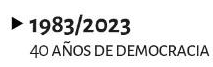
\includegraphics[scale=0.4]{año.PNG}\end{tabular}}
\fancyfoot[R]{\thepage}
\fancyfoot[C]{\begin{tabular}{@{}c@{}}\textbf{BORQUEZ PEREZ Juan Manuel}\\ \textbf{Legajo 13567}\end{tabular}}
\renewcommand{\footrulewidth}{0.2pt}

\begin{document}

\begin{titlepage}
    \centering
    \vspace*{5cm}
    {\Huge\bfseries Informe de Trabajo Práctico}\\
    \vspace{0.2cm}
    {\Large \textbf{N°1 - Parte C: Fundamentos -  Herencia, agregación, polimorfismo }}\\
    \vspace{0.5cm}
    {\Large Programación Orientada a Objetos}\\
    \vspace{0.2 cm}
    {\Large Ingeniería en Mecatrónica}\\
    \vspace{1.5cm}
    Alumno: Juan Manuel BORQUEZ PEREZ\\
    Legajo: 13567\\
    \vfill
    {\begin{tabular}{@{}c@{}}
\includegraphics[scale=0.4]{escudo.PNG}\end{tabular}}\hspace{10pt}
    {\begin{tabular}{@{}c@{}}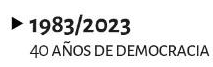
\includegraphics[scale=0.6]{año.PNG}\end{tabular}}
    %Año 2023
\end{titlepage}
\section{Enunciado}
\begin{itemize}
    \item[a)] Prepare un directorio denominado \texttt{apellido\_legajo\_C} (reemplace con sus datos) que contenga 2 subdirectorios denominados \texttt{cons\_4} y \texttt{cons\_5}.
    \item[b)] Ubique en cada uno de ellos la implementación que corresponda según la consigna.
    \item[c)] Coloque en el directorio raíz (\texttt{apellido\_legajo\_C}) el documento con el informe general para esta entrega (siga el mismo formato de la anterior).
    \item[d)] Al finalizar, suba un archivo comprimido de la carpeta raíz creada (incluyendo todo su contenido) en la actividad denominada Entrega C, dentro del aula virtual.
    \item[e)] En cada consigna, Usted debe diseñar un modelo orientado a objetos que incorpore las clases mínimas indicadas e informarlo mediante un diagrama de clases.
    \item[f)] Fecha de entrega: 20 de setiembre de 2023.
\end{itemize}

\subsection{Consigna 4}
Implementar en lenguaje Python, bajo el paradigma orientado a objetos, un programa de utilidad que ofrezca un menú de usuario con la siguiente funcionalidad:
\begin{itemize}
    \item Listar los archivos de arte ASCII disponibles en un directorio ubicado en el espacio de la aplicación.
    \item Seleccionar un archivo en particular mediante el tipeado de su nombre completo.
    \item Visualizar en la consola el contenido del archivo con el arte ASCII que contiene y un informe de análisis del mismo. Este informe debe indicar:
    \begin{itemize}
        \item Qué caracteres se usaron en el archivo de arte ASCII.
        \item Cuántos caracteres hay de cada uno y el total.
    \end{itemize}
    \item Listar, en formato JSON, las coordenadas (solamente) que corresponden a un carácter indicado por el operador, considerando que [0, 0] se encuentra en la esquina superior izquierda.
    \item \textbf{[Desarrollo opcional]} Obtener la línea de texto del mensaje sin formato y su longitud, usando subprocesos y el binario del generador de arte ASCII.
    \item Terminar la ejecución.
\end{itemize}
\subsubsection{Observaciones y restricciones al diseño e implementación.}

\begin{itemize}
    \item Algunos archivos de prueba, para colocar dentro del directorio ya mencionado, se encuentran en el aula virtual (denominados \texttt{ejemploN.txt}), sin embargo, usted puede agregar otros si lo cree conveniente. Para ello, puede usar el generador provisto (denominado \texttt{c4ascii.cpp}).
    \item Los archivos de arte ASCII responden al siguiente formato interno:
    \begin{itemize}
        \item Contenido como texto plano.
        \item 7 filas de \(N\) caracteres ASCII, dependiendo \(N\) de la longitud de la línea con el mensaje.
        \item Un carácter de frente (para el texto del mensaje) y un carácter de fondo
        \item Por ejemplo:
        
        \begin{figure}[!h]
        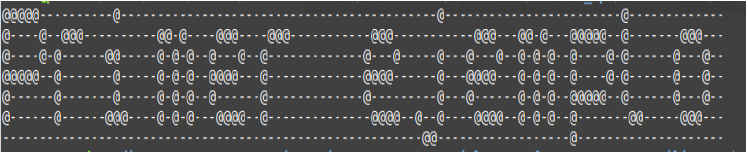
\includegraphics[width = \textwidth]{C4/Ejemplo_consigna.PNG}
        \end{figure}
        
    \end{itemize}
    \item Actualmente, el generador admite 1 carácter de frente; sin embargo, se estima que su funcionalidad será ampliada para usar diferentes caracteres.
    \item Las opciones de visualización e informe no deben operar sobre el sistema de archivos.
    \item El aplicativo debe ofrecer mensajes de ayuda cuando ocurran situaciones no previstas o el usuario seleccione una opción que dependa de otra.
    \item Aplique un esquema de diseño que separe la capa de modelo de las de vista y control.
    \item Para el manejo de errores y excepciones, utilizar subclases de Exception.
    \item Para la interfaz de usuario, usar formato CLI y reutilización mediante herencia.
    \item Incluya en su modelo OO las siguientes clases, agregando aquellos elementos que considere adecuados:
\end{itemize}
\begin{figure}[!h]
        \centering
        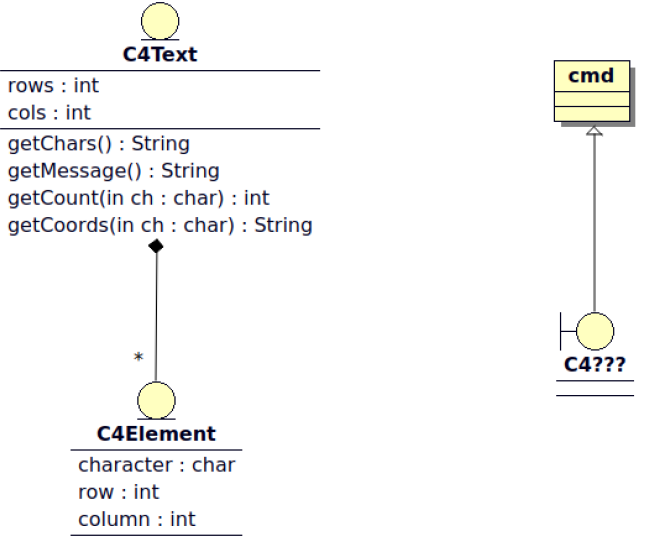
\includegraphics[scale=0.5]{C4/Diagrama_de_Clases_C4.PNG}
\end{figure}

\subsection{Consigna 5}

Utilizando UML para representar el modelo orientado a objetos y el lenguaje C++ para la implementación, desarrolle una pequeña herramienta para su uso en un sistema de comunicaciones en red conforme al requerimiento descripto:

\begin{itemize}
    \item La aplicación deseada sigue una arquitectura cliente/servidor.
    \begin{itemize}
        \item Los valores son puestos a disposición de los clientes mediante XML-RPC en un port específico para una IP dinámica, que se informa al momento del lanzamiento del servidor.
        \item No se requiere una interfaz de usuario especial. Es una herramienta del tipo orden o comando del sistema(tanto para el servidor como para el cliente). Esto implica considerar el uso de argumentos de línea de comandos.
    \end{itemize}
    \item El servidor debe proveer los siguientes servicios:
    \begin{itemize}
        \item Validar cada petición en base a un identificador de usuario.
        \item Permitir a un usuario iniciar un proceso de generación de números.
        \item Generar un número real con 2 dígitos de precisión en un rango [-CI, CS], donde CI y CS son los valores paramétricos de las cotas superior e inferior del rango, recibidos desde el cliente.
        \item Generar un número entero en un rango [-CI, CS] proporcionado por el cliente.
        \item Informar el valor de un número generado por el usuario, con su marca de tiempo y el rango asociados.
        \item Informar la cantidad de números generados por el usuario, su suma total y su promedio.
        \item Listar los números generados por el usuario remoto desde que inició el proceso de generación, incluyendo el tipo, el instante de tiempo en que se generó, el rango de cada uno y, al final, el tiempo que llevó realizar todo el proceso desde que se hizo la primera solicitud.
    \end{itemize}
    \item El cliente debe permitir:
    \begin{itemize}
        \item Solicitar un número entero en un rango indicado explícitamente.
        \item Solicitar un número real en un rango indicado explícitamente.
        \item Solicitar un número entero sin indicar el rango. En este caso, el servidor utiliza el mismo rango de la petición entera anterior.
        \item Solicitar un número real sin especificar el rango. En este caso, el servidor utiliza el mismo rango de la petición real anterior.
        \item Solicitar la información asociada a un número generado anteriormente. En este caso, la petición se realiza enviando el ordinal deseado.
        \item Solicitar la estadística básica.
        \item Solicitar el listado de números generados.
        \item Mostrar en pantalla cada respuesta obtenida.
        \item Guardar la respuesta obtenida en un archivo con formato XML bien formado. El nombre del archivo se provee en cada petición.
    \end{itemize}
\end{itemize}

\subsubsection{Observaciones y restricciones al diseño e implementación.}
\begin{itemize}
    \item Si bien son pocos usuarios, cada uno se identifica por un número de 3 dígitos.
    \item Los identificadores de los usuarios habilitados se encuentran almacenados en un archivo de texto predefinido del lado servidor.
    \item Un usuario puede acceder solo a los datos generados por él.
    \item La marca de tiempo de generación de cada número corresponde a la cantidad de segundos desde que el usuario inició el proceso.
    \item Contemplar el control de errores en los escenarios básicos de operación usando excepciones.
    \item Incluya los mensajes al usuario que correspondan, así como ayudas de operación o notificación de errores.
    \item Aplique un diseño de 2 capas con separación entre el modelo y la presentación/control.
    \item Por simplicidad, se sugiere el uso de la librería XML-RPC para C++, disponible desde la URL \url{http://xmlrpcpp.sourceforge.net/}. Considere la lectura de la documentación disponible en la página del proyecto. Revise el video explicativo de clase, sobre el montaje de un aplicativo C/S usando dicha librería, en \url{https://youtu.be/B4vzzSqODvA} (aproximadamente desde 4:40 minutos). Puede ver un aplicativo similar en \url{https://youtu.be/2an54kpvg3c}. Sin embargo, queda a su preferencia el uso de una librería similar.
    \item Incluya en su modelo OO las siguientes clases, además de cualquier otro elemento que considere adecuado:
\end{itemize}
\begin{figure}[!h]
        \centering
        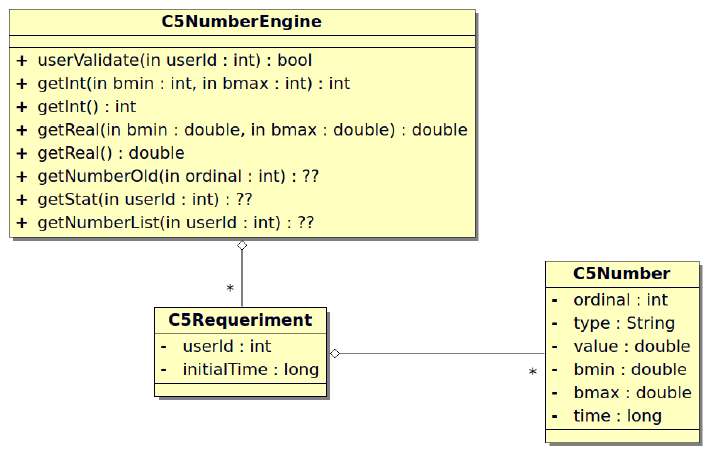
\includegraphics[scale=0.5]{C5/Diagrama_de_Clases_C5.PNG}
\end{figure}


\section{Esquema General de la Solución}
%Esquema general de la solución: representación gráfica con el diseño del modelo lógico.
\subsection{Consigna 4}
Esquema lógico general de la solución para la consigna 4.

La mayoría de la información relativa a las clases mostradas en el siguiente esquema está indicada como comentarios en los métodos y descripciones de las clases. A continuación, se realiza una descripción general de la solución:

\begin{itemize}
    \item La clase `main` representa el archivo principal de la solución.
    \item `C4` es la principal clase de la solución que tiene los métodos CLI y permite la interacción con el usuario a través de prompts y salidas por pantalla.
    \item Los objetos de la clase `C4File` están asociados a archivos de arte ASCII particulares. Se trata de objetos temporales utilizados únicamente durante la construcción de los objetos de la clase `C4Text` para realizar la lectura de los archivos de arte ASCII.
    \item Los objetos de la clase `C4Text` son representaciones del arte ASCII contenida en los archivos. Permiten acceder a información y operaciones generales de los mismos.
    \item Los objetos de la clase `C4Element` son objetos persistentes contenidos dentro de objetos de la clase `C4Text`.
    \item `asciiGenerator` es una clase con información y un método particular para el acceso al procedimiento remoto de la aplicación de ASCII art auxiliar. Tiene información de clase persistente común a todos los objetos de esta clase. Cada objeto se crea con el propósito de acceder al método.
\end{itemize}

\begin{figure}[!h]
    \centering
    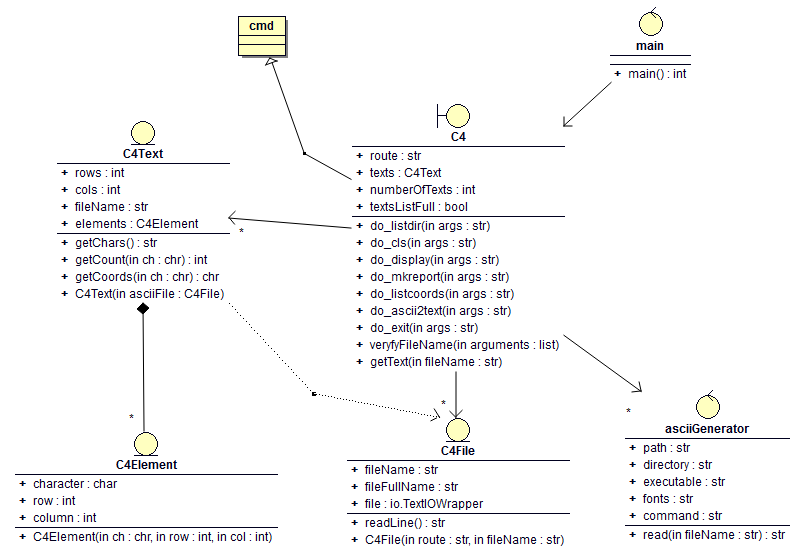
\includegraphics[width=\dimexpr\textwidth]{C4/Esquema_general_C4.PNG}
\end{figure}
\newpage
\subsection{Consigna 5}
Esquema lógico general de la solución para la consigna 5

La mayoría de la información relativa a las clases mostradas en los siguiente esquema está indicada como comentarios en los métodos y
descripciones de las clases. A continuación, se realiza una descripción general de la solución:

Se llevó a cabo un diagrama de clases para la parte del cliente y varios diagramas para la parte del servidor.
Todos los diagramas y la distribución general de la aplicación, junto con las relaciones, se pueden acceder desde el proyecto de UML
que se encuentra en la carpeta UML dentro de la consigna 5 en \path{./cons_5/C5/UML/C5}.
El diagrama para la parte del cliente es menos cargado y se presenta en una sola captura en la figura \ref{fig:cliente},
a la que se puede acceder desde el panel de navegación en BOUML como se indica en la captura \ref{fig:navegacion_cliente}.

La parte del servidor implica un conjunto de relaciones más complejas y en mayor cantidad si se tienen en cuenta todas las modificaciones realizadas.
El diagrama completo para la parte del servidor no se presenta de forma legible en una sola captura (ver figura \ref{fig:servidor}) y,
por lo tanto, se decidió armar varios diagramas de clases para las partes más importantes del servidor.
A estos diagramas se puede acceder desde el panel de navegación en UML como se indica en la captura \ref{fig:navegacion_servidor}.

Por un lado, en la figura \ref{fig:relaciones_principales} se encuentra el diagrama que representa las relaciones entre las clases principales dadas en la consigna.
El diagrama que se muestra en las figuras \ref{fig:excepciones_personalizadas1} y \ref{fig:excepciones_personalizadas2}
representa las relaciones entre clases asociadas a las excepciones personalizadas que se han definido
Las figuras \ref{fig:relaciones_rpc1} y \ref{fig:relaciones_rpc2} representan las relaciones entre clases asociadas al servidor RPC.

\begin{figure}[htbp]
    \centering
    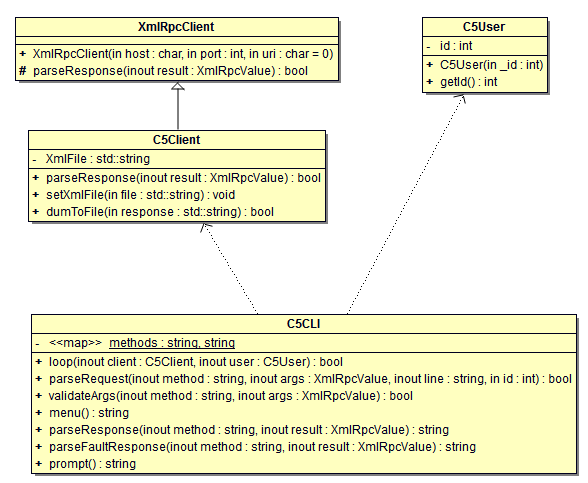
\includegraphics[width=\textwidth]{C5/Esquema_general_C5_cliente.PNG}
    \caption{Diagrama de clases para la parte del cliente.}
    \label{fig:cliente}
\end{figure}

\begin{figure}[htbp]
    \centering
    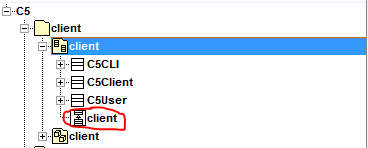
\includegraphics[width=0.5\textwidth]{C5/Esquema_general_C5_cliente_panel.PNG}
    \caption{Captura del panel de navegación en BOUML para acceder al diagrama del cliente.}
    \label{fig:navegacion_cliente}
\end{figure}

\begin{figure}[htbp]
    \centering
    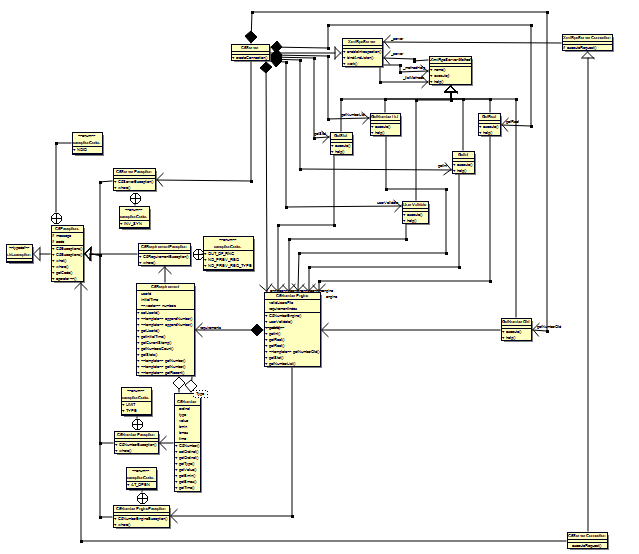
\includegraphics[width=\textwidth]{C5/Esquema_general_C5_server_todo.PNG}
    \caption{Diagrama completo para la parte del servidor.}
    \label{fig:servidor}
\end{figure}

\begin{figure}[htbp]
    \centering
    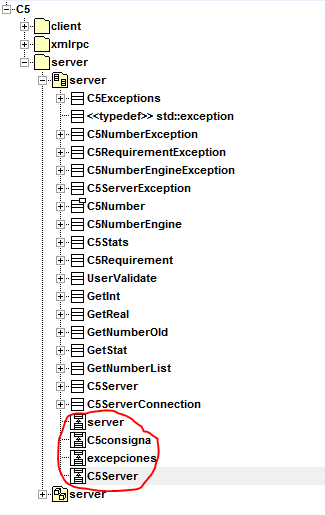
\includegraphics[width=0.5\textwidth]{C5/Esquema_general_C5_server_panel.PNG}
    \caption{Captura del panel de navegación en UML para acceder a los diagramas del servidor.}
    \label{fig:navegacion_servidor}
\end{figure}

\begin{figure}[htbp]
    \centering
    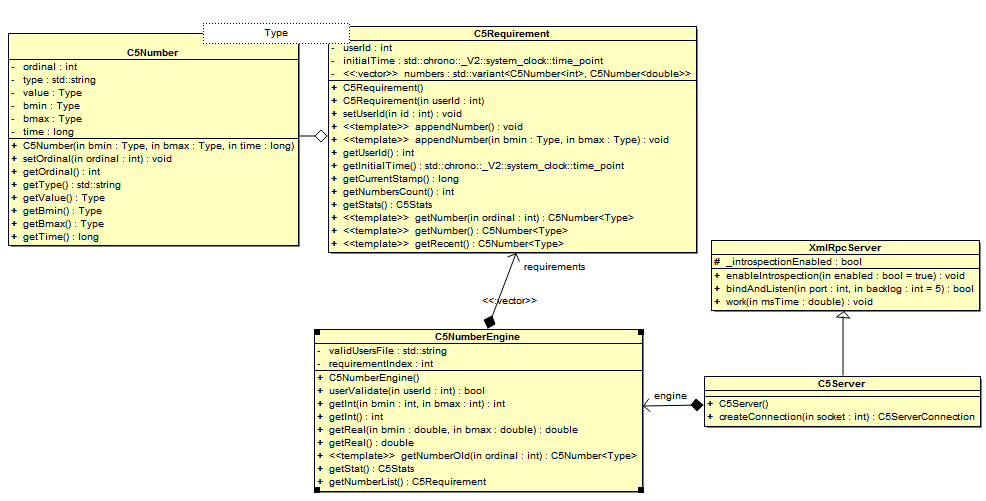
\includegraphics[width=\textwidth]{C5/Esquema_general_C5_server_consigna.PNG}
    \caption{Diagrama de relaciones entre las clases principales.}
    \label{fig:relaciones_principales}
\end{figure}

\begin{figure}[htbp]
    \centering
    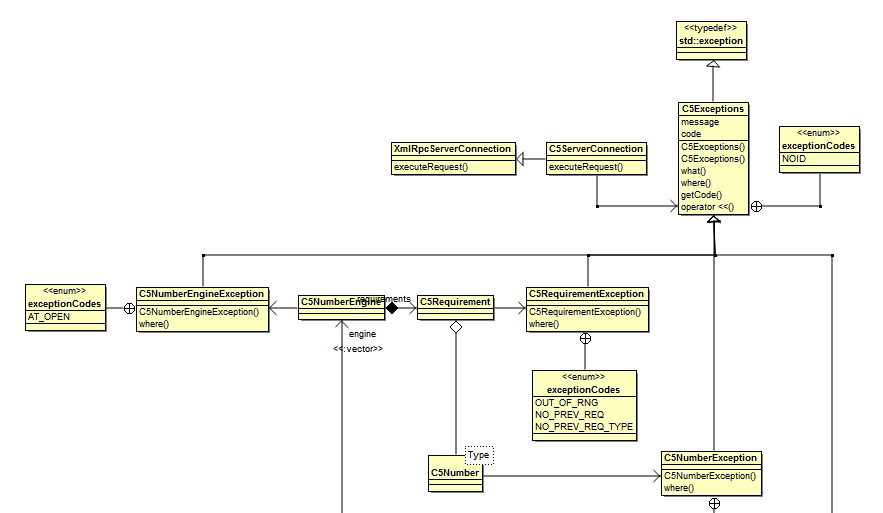
\includegraphics[width=\textwidth]{C5/Esquema_general_C5_server_excepciones_1.PNG}
    \caption{Diagrama de relaciones entre clases asociadas a excepciones personalizadas.}
    \label{fig:excepciones_personalizadas1}
\end{figure}

\begin{figure}[htbp]
    \centering
    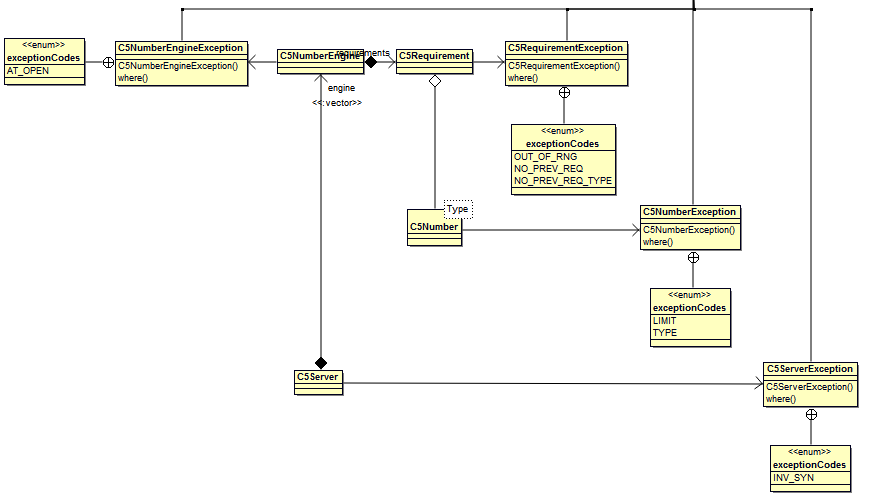
\includegraphics[width=\textwidth]{C5/Esquema_general_C5_server_excepciones_2.PNG}
    \caption{Diagrama de relaciones entre clases asociadas a excepciones personalizadas.}
    \label{fig:excepciones_personalizadas2}
\end{figure}

\begin{figure}[htbp]
    \centering
    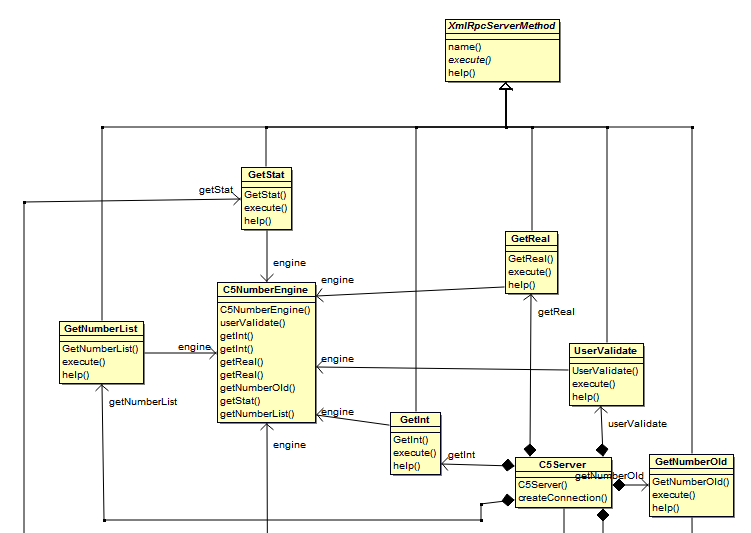
\includegraphics[width=\textwidth]{C5/Esquema_general_C5_server_server_1.PNG}
    \caption{Diagrama de relaciones entre clases asociadas al servidor RPC.}
    \label{fig:relaciones_rpc1}
\end{figure}

\begin{figure}[htbp]
    \centering
    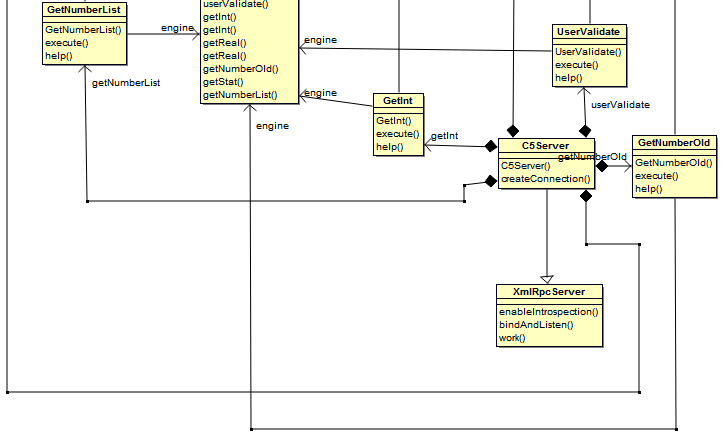
\includegraphics[width=\textwidth]{C5/Esquema_general_C5_server_server_2.PNG}
    \caption{Diagrama de relaciones entre clases asociadas al servidor RPC.}
    \label{fig:relaciones_rpc2}
\end{figure}

\newpage
\section{Interfaces de Usuario}
\subsection{Consigna 4}
%Interfaces de usuario: captura de pantallas de entrada/salida resultantes para una ejecución completa.
Secuencia de capturas para una ejecución completa y sin errores.


\begin{figure}[htbp]
    \centering
    \begin{adjustbox}{max width=\textwidth, center}
        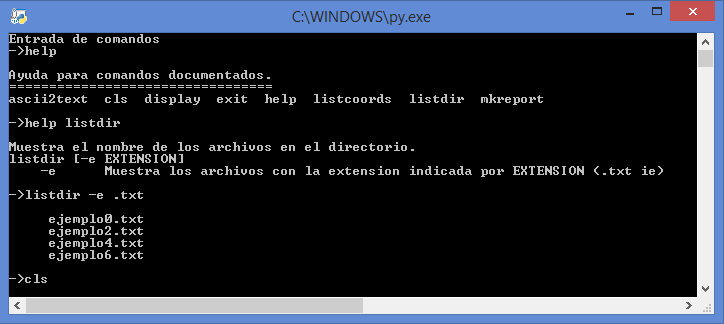
\includegraphics{C4/S1_C4.PNG}
    \end{adjustbox}
    \begin{adjustbox}{max width=\textwidth, center}
        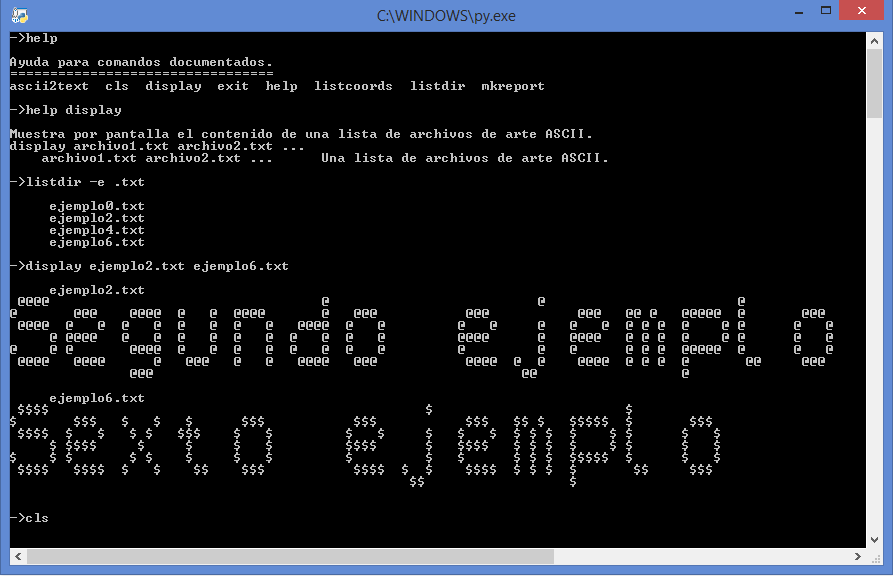
\includegraphics{C4/S2_C4.PNG}
    \end{adjustbox}
\end{figure}

\begin{figure}[htbp]
    \centering
    \begin{adjustbox}{max width=\textwidth, center}
        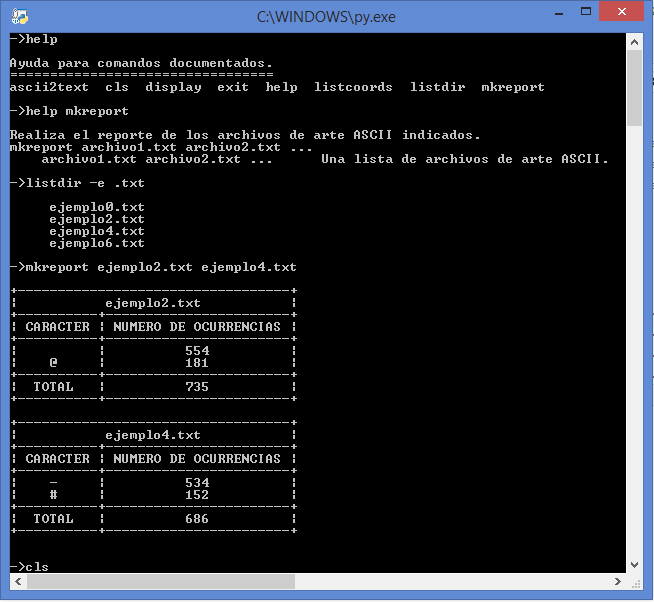
\includegraphics{C4/S3_C4.PNG}
    \end{adjustbox}
\end{figure}
\begin{figure}[htbp]
    \begin{adjustbox}{max width=\textwidth}
        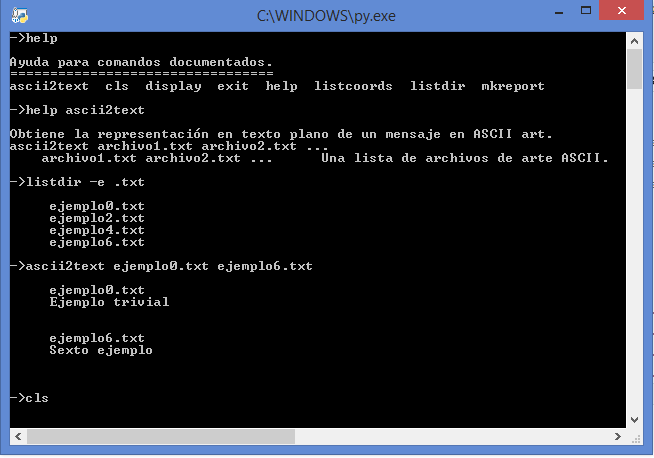
\includegraphics{C4/S4_C4.PNG}
    \end{adjustbox}
\end{figure}
\clearpage
\begin{figure}[htbp]
    \begin{adjustbox}{max width=\textwidth, center}
        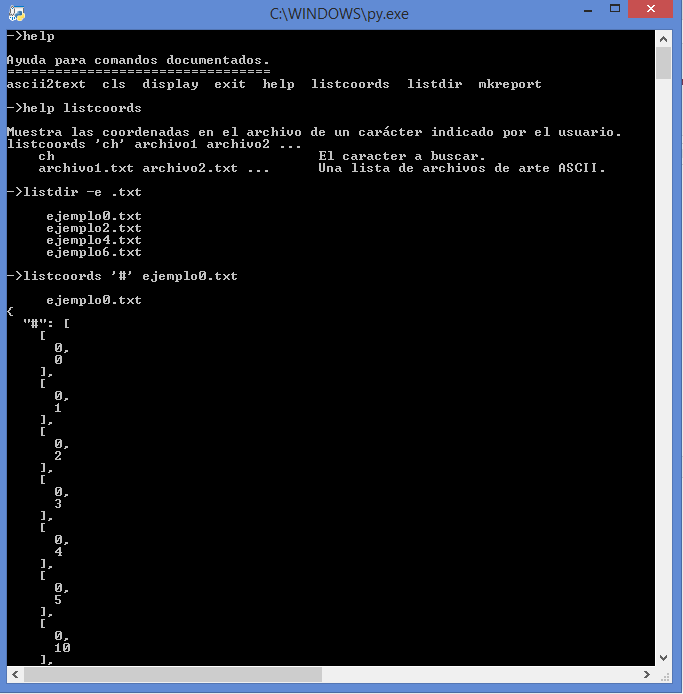
\includegraphics{C4/S5_C4.PNG}
    \end{adjustbox}
\end{figure}
\begin{figure}[htbp]
    \begin{adjustbox}{max width=\textwidth, center}
        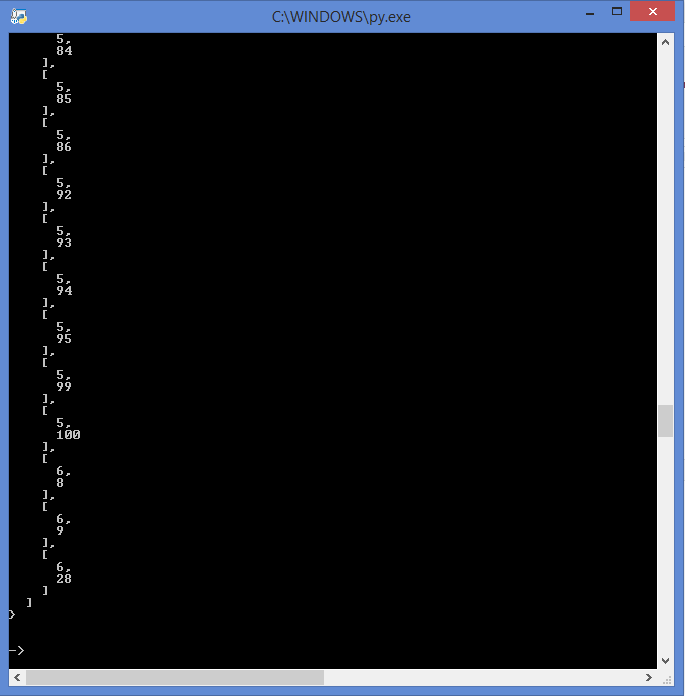
\includegraphics{C4/S6_C4.PNG}
    \end{adjustbox}
\end{figure}
\begin{figure}[htbp]
    \begin{adjustbox}{max width=\textwidth, center}
        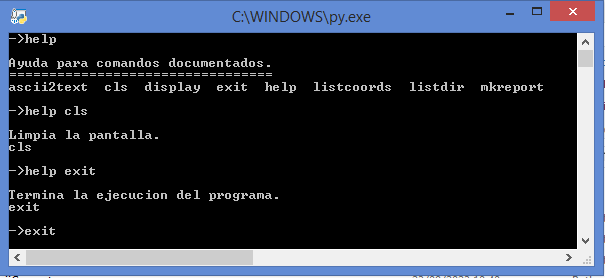
\includegraphics{C4/S7_C4.PNG}
    \end{adjustbox}
\end{figure}

\newpage
\subsection{Consigna 5}
Secuencia de Capturas para una ejecución completa y sin errores.

En las captura, en la parte derecha se muestra la ventana del cleinte y en
la parte izquierda la ventana del servidor. En este caso la verbosidad del servidor
está seteada en su máximo valor (5).
\begin{figure}[htbp]
    \centering
    \begin{adjustbox}{max width=\textwidth, center}
        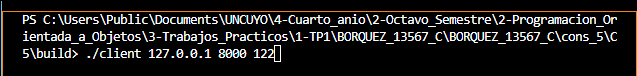
\includegraphics{C5/Linea_ejecucion_cliente.PNG}
    \end{adjustbox}
\end{figure}
\begin{figure}[htbp]
    \centering
    \begin{adjustbox}{max width=\textwidth, center}
        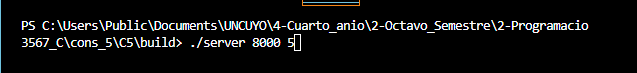
\includegraphics{C5/Linea_ejecucion_servidor.PNG}
    \end{adjustbox}
\end{figure}
\begin{figure}[htbp]
    \centering
    \begin{adjustbox}{max width=\textwidth, center}
        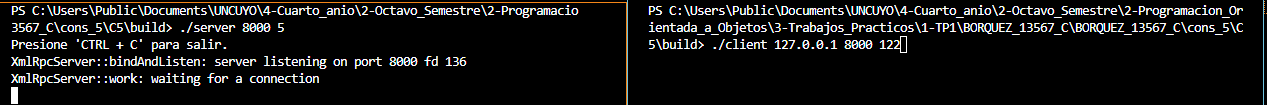
\includegraphics{C5/Servidor_cliente_1.PNG}
    \end{adjustbox}
\end{figure}
\begin{figure}[htbp]
    \centering
    \begin{adjustbox}{max width=\textwidth, center}
        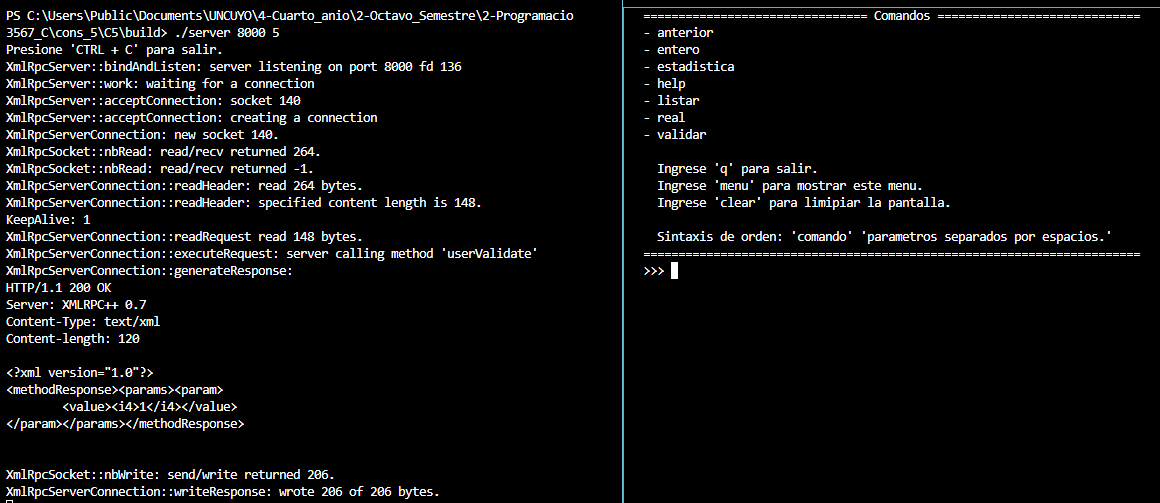
\includegraphics{C5/Servidor_cliente_2.PNG}
    \end{adjustbox}
\end{figure}
\begin{figure}[htbp]
    \begin{adjustbox}{max width=\textwidth, center}
        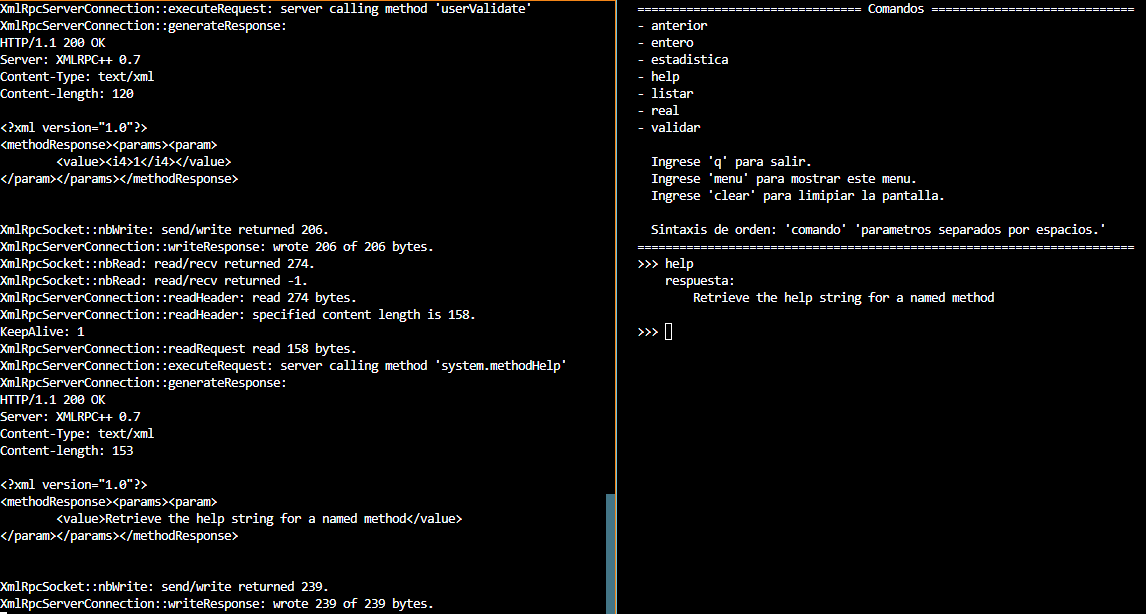
\includegraphics{C5/Servidor_cliente_3.PNG}
    \end{adjustbox}
\end{figure}
\begin{figure}[htbp]
    \begin{adjustbox}{max width=\textwidth, center}
        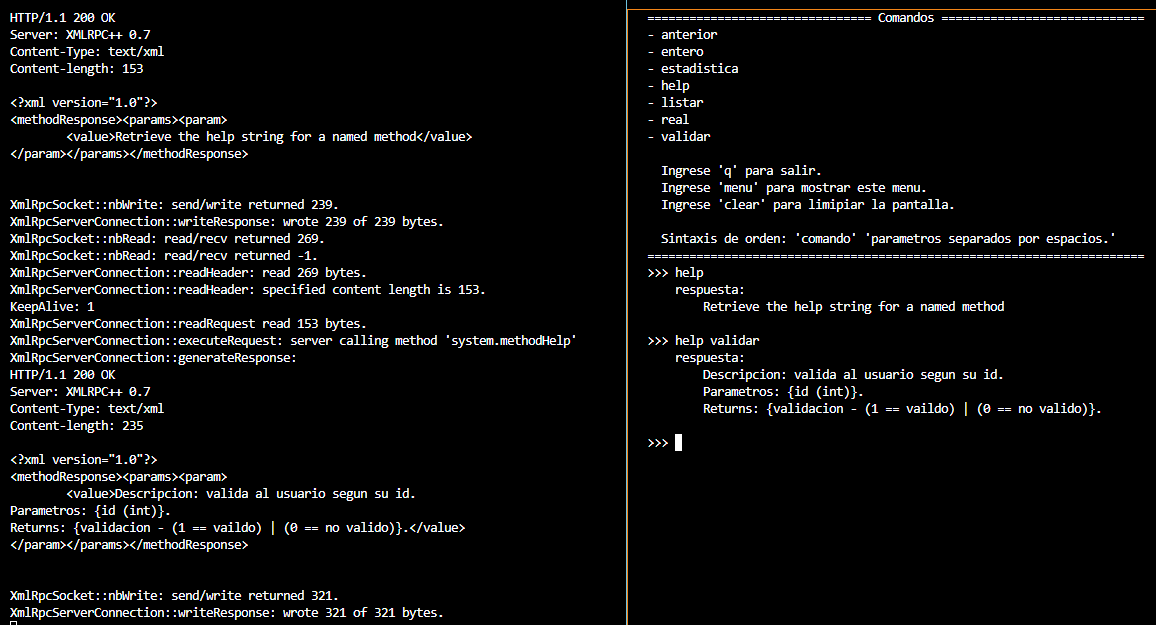
\includegraphics{C5/Servidor_cliente_4.PNG}
    \end{adjustbox}
\end{figure}
\begin{figure}[htbp]
    \begin{adjustbox}{max width=\textwidth, center}
        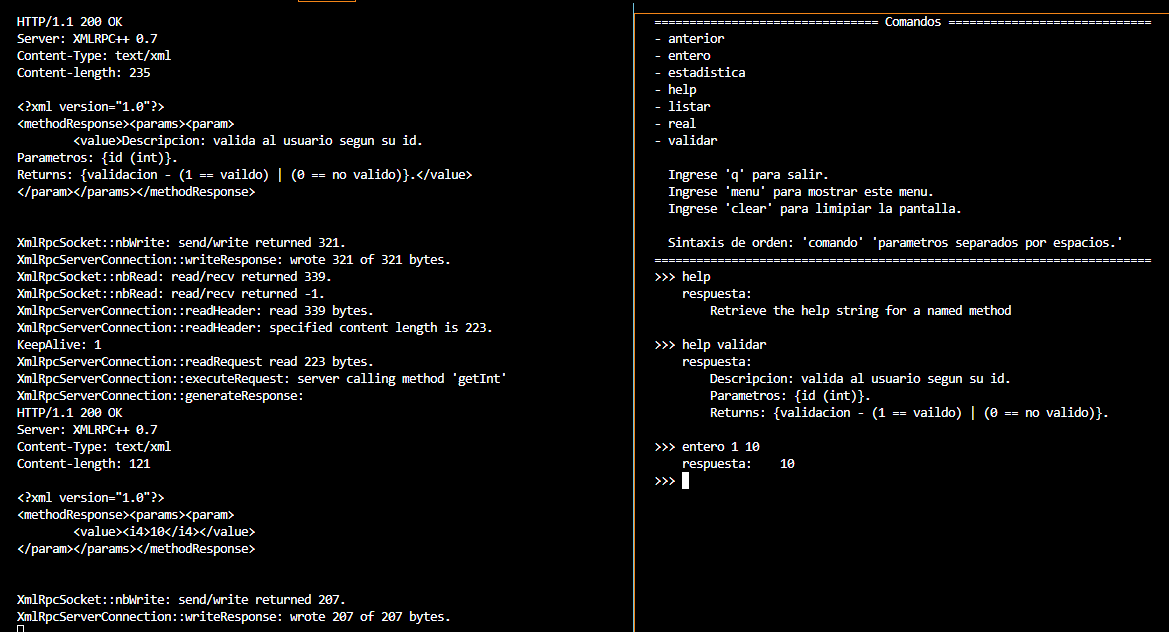
\includegraphics{C5/Servidor_cliente_5.PNG}
    \end{adjustbox}
\end{figure}
\begin{figure}[htbp]
    \begin{adjustbox}{max width=\textwidth, center}
        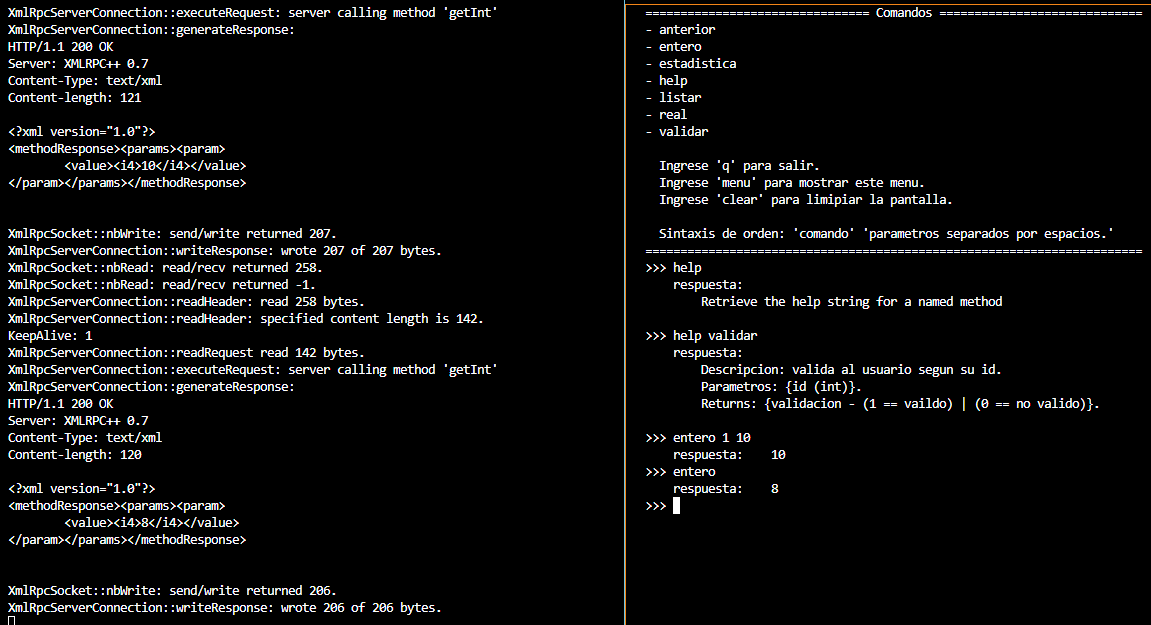
\includegraphics{C5/Servidor_cliente_6.PNG}
    \end{adjustbox}
\end{figure}
\begin{figure}[htbp]
    \begin{adjustbox}{max width=\textwidth, center}
        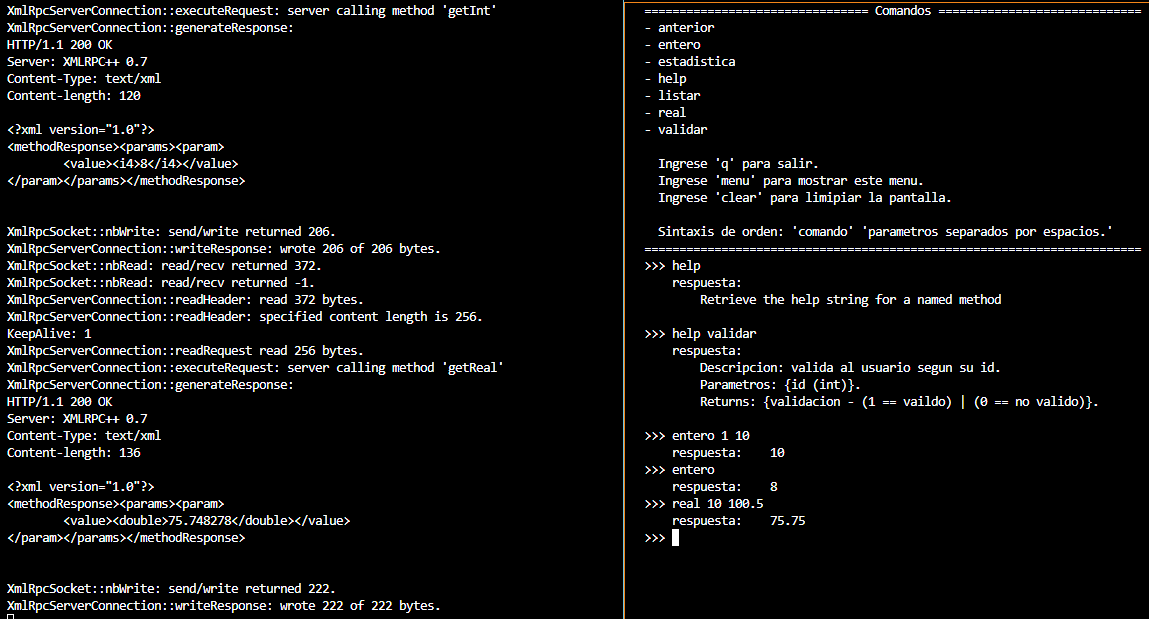
\includegraphics{C5/Servidor_cliente_7.PNG}
    \end{adjustbox}
\end{figure}
\begin{figure}[htbp]
    \begin{adjustbox}{max width=\textwidth, center}
        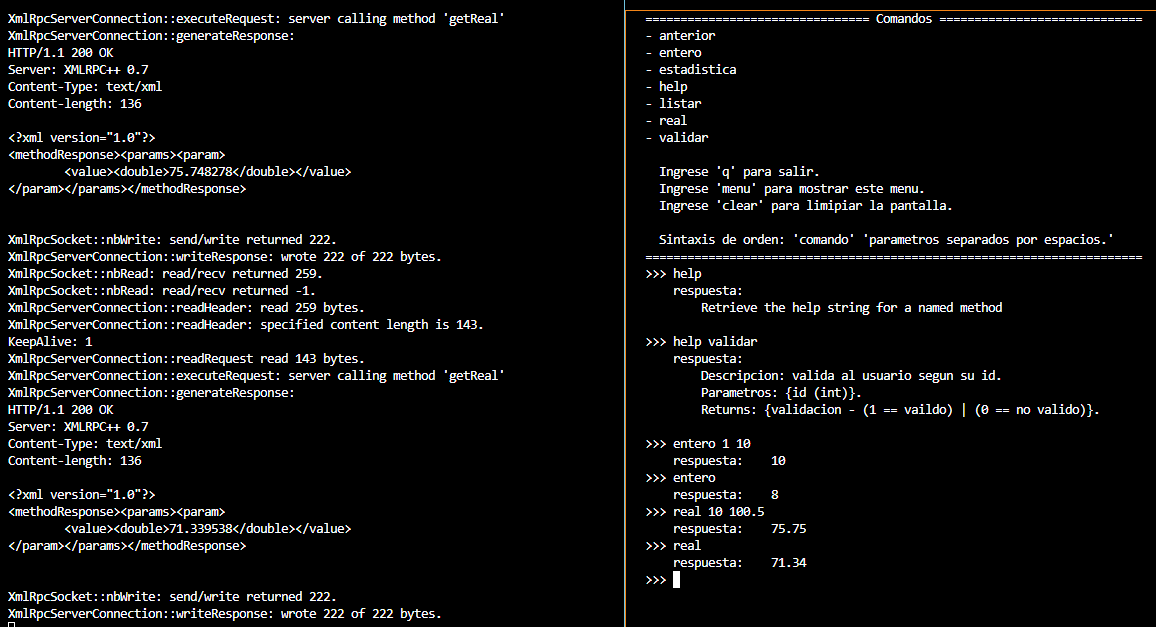
\includegraphics{C5/Servidor_cliente_8.PNG}
    \end{adjustbox}
\end{figure}
\begin{figure}[htbp]
    \begin{adjustbox}{max width=\textwidth, center}
        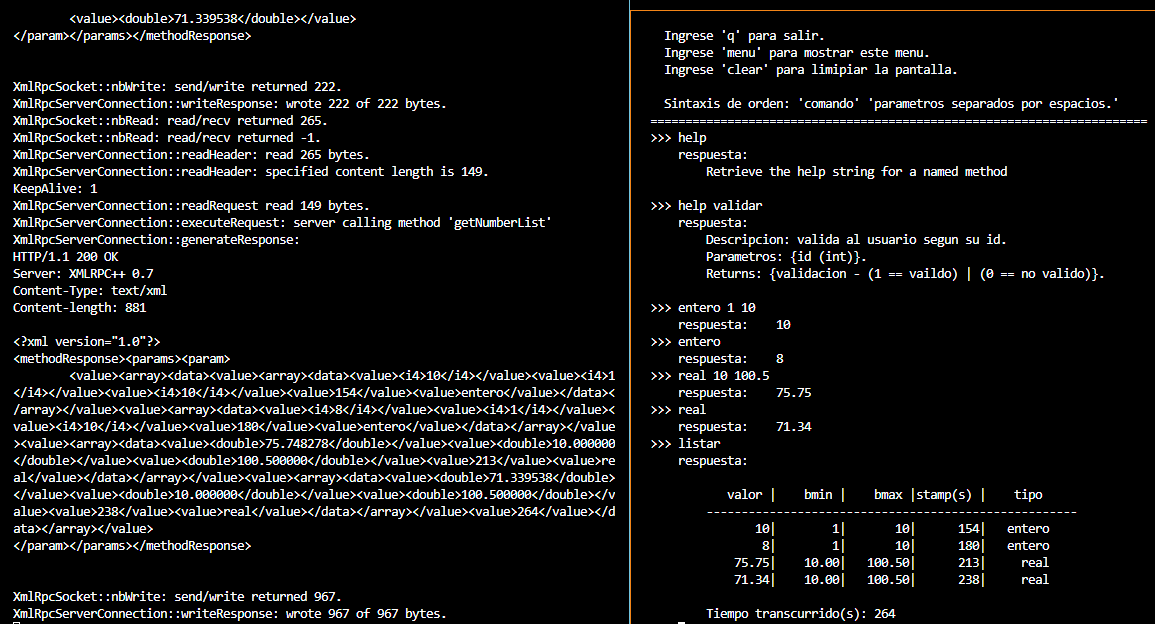
\includegraphics{C5/Servidor_cliente_9.PNG}
    \end{adjustbox}
\end{figure}
\begin{figure}[htbp]
    \begin{adjustbox}{max width=\textwidth, center}
        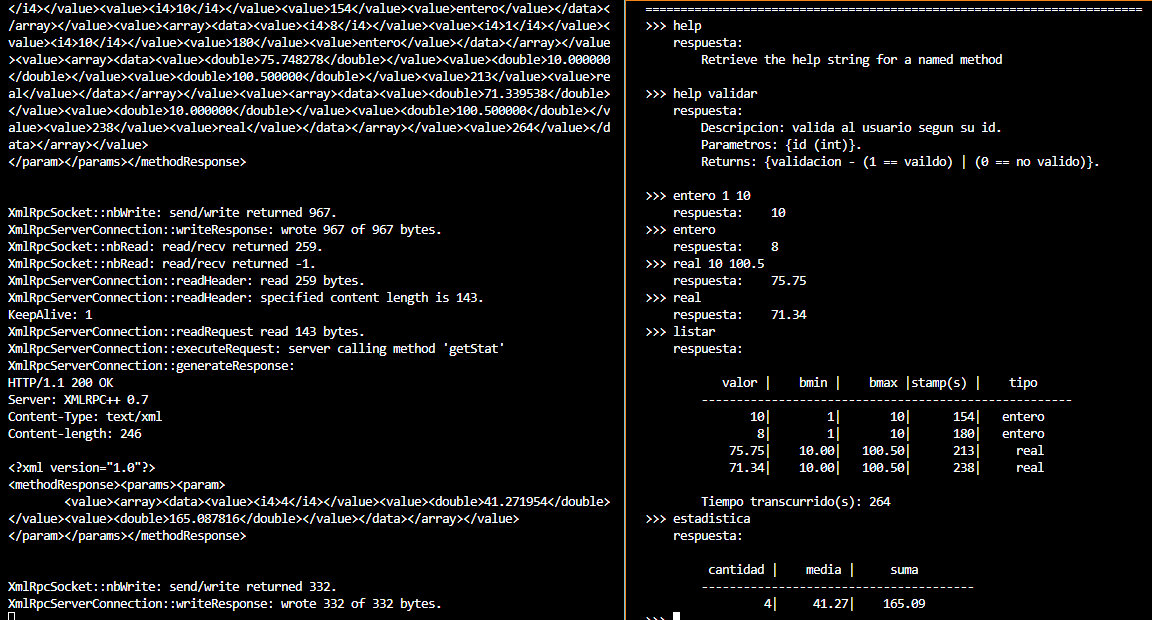
\includegraphics{C5/Servidor_cliente_10.PNG}
    \end{adjustbox}
\end{figure}
\begin{figure}[htbp]
    \begin{adjustbox}{max width=\textwidth, center}
        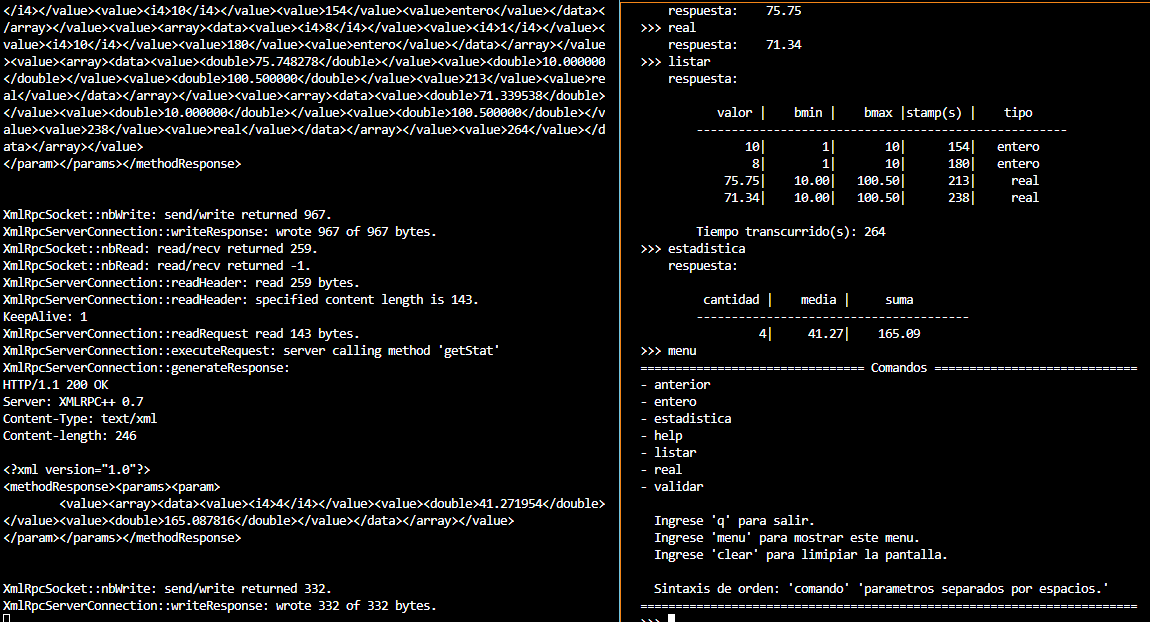
\includegraphics{C5/Servidor_cliente_11.PNG}
    \end{adjustbox}
\end{figure}
\begin{figure}[htbp]
    \begin{adjustbox}{max width=\textwidth, center}
        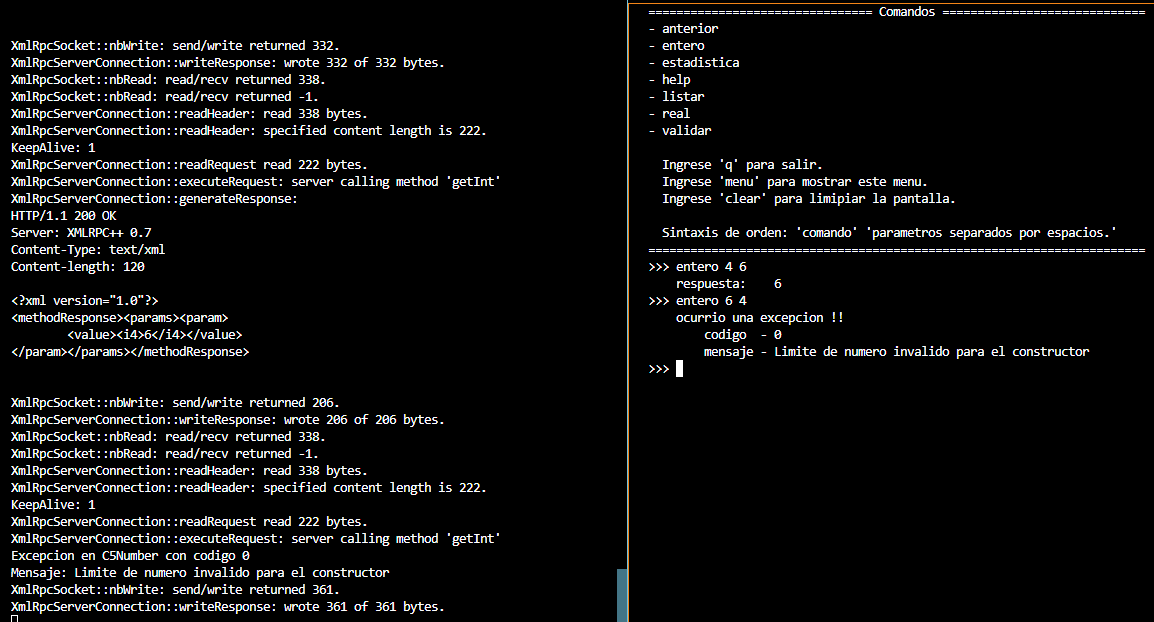
\includegraphics{C5/Servidor_cliente_12.PNG}
    \end{adjustbox}
\end{figure}
\begin{figure}[htbp]
    \begin{adjustbox}{max width=\textwidth, center}
        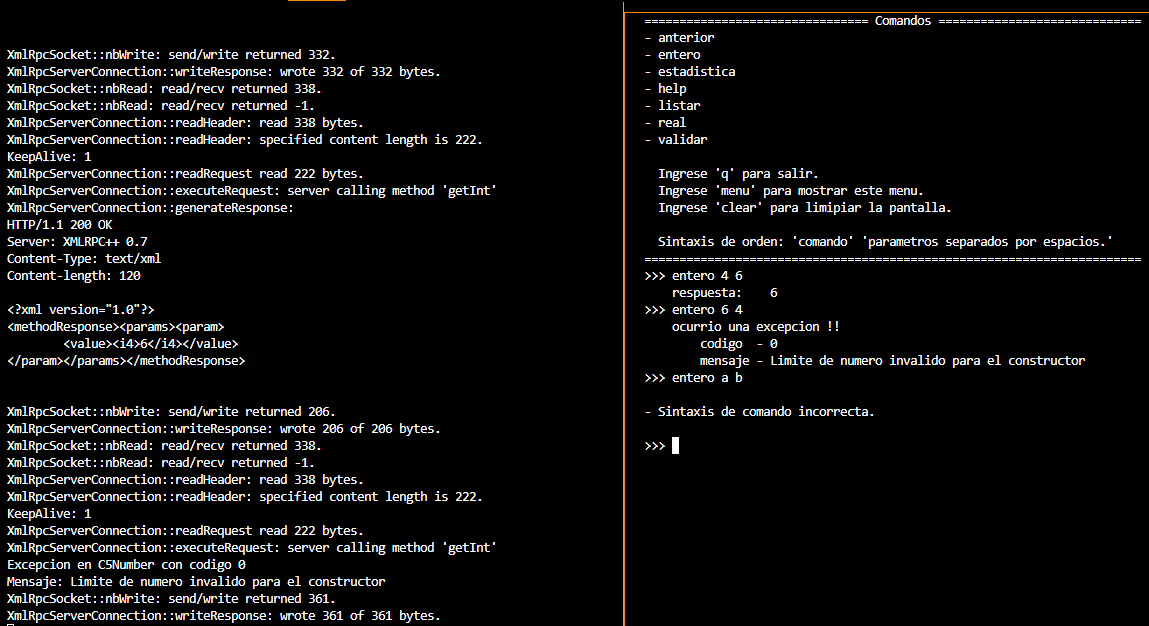
\includegraphics{C5/Servidor_cliente_13.PNG}
    \end{adjustbox}
\end{figure}
\begin{figure}[htbp]
    \begin{adjustbox}{max width=\textwidth, center}
        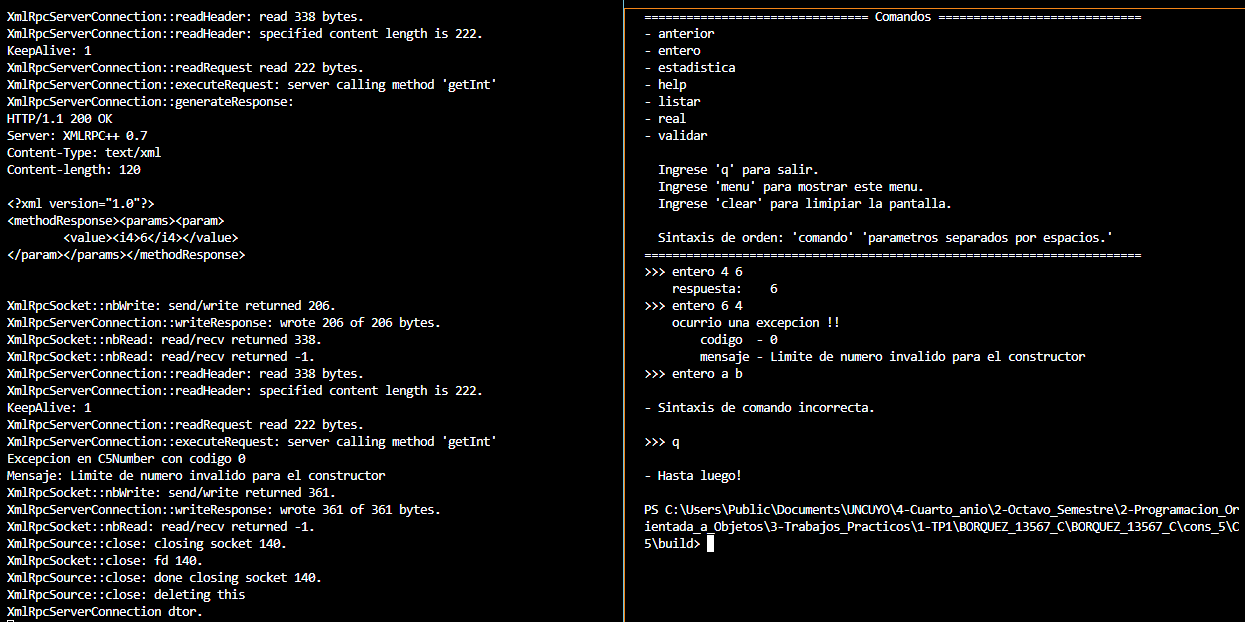
\includegraphics{C5/Servidor_cliente_14.PNG}
    \end{adjustbox}
\end{figure}
\newpage
\section{Uso}
%Uso: descripción de las consideraciones a tener en cuenta por un usuario que desea hacer uso del aplicativo resultante y/o reutilizar su código.

\subsection{Consigna 4}
La aplicación se ejecuta abriendo el archivo "main.py".

La aplicación asociada a esta consigna permite el tratamiento general de archivos con arte ASCII. Presenta una interfaz de línea de comandos que permite al usuario llevar a cabo distintas operaciones mediante comandos.

Las operaciones que se pueden realizar con archivos de arte ASCII están documentadas. Puedes acceder a esta documentación de ayuda para cada comando utilizando el comando "help" sin parámetros, que lista todos los comandos disponibles, o utilizando el mismo comando seguido del nombre de un comando específico para acceder a ayuda específica para ese comando ("help comando").

A continuación, se indican las operaciones que se pueden llevar a cabo:

\begin{itemize}
    \item \textbf{listdir}: Muestra los nombres de los archivos en el directorio de la aplicación. También puedes listar aquellos con una extensión específica, por ejemplo, .txt para arte ASCII.
    \item \textbf{display}: Muestra por pantalla el contenido de una lista de archivos de arte ASCII.
    \item \textbf{mkreport}: Genera un reporte del contenido del archivo de arte ASCII, incluyendo los caracteres utilizados y el número de ocurrencias.
    \item \textbf{listcoords}: Muestra las coordenadas en las que se presenta un carácter específico dentro de un archivo de arte ASCII.
    \item \textbf{ascii2text}: Convierte el contenido de un archivo de arte ASCII en un mensaje en texto plano.
    \item \textbf{cls}: Limpia la pantalla.
    \item \textbf{exit}: Termina la ejecución.
\end{itemize}

Para que la aplicación funcione correctamente, es importante que todos los archivos de código se encuentren en el mismo directorio tal como se entregan. Además, el módulo auxiliar en C++ utilizado para el tratamiento de archivos de arte ASCII, el cual se usa para la traducción del contenido de arte ASCII a un mensaje en texto plano, debe estar contenido en la carpeta especificada dentro del directorio de la solución, junto con el archivo "font.txt". En resumen, la disposición de archivos en directorios debe ser la misma que se proporciona con la aplicación.

El manejo de errores se realiza principalmente en los métodos de comandos de la clase C4. En los demás módulos, se lanzan excepciones en casos específicos. Aprovechamos el sistema para la validación de archivos, por lo que no realizamos explícitamente una verificación de la existencia de un archivo. En su lugar, al intentar abrir un archivo que no existe, capturamos la excepción generada por el sistema.


\subsection{Consigna 5}
Una explicación detallada sobre el uso de la aplicación se puede encontrar en el archivo
\texttt{README.txt} ubicado en la carpeta de la solución en \texttt{cons\_5/C5}. Del mismo modo, durante la ejecución,
se proporcionan instrucciones de ayuda al usuario que utiliza la interfaz de línea de comandos (CLI).

En relación con la extensión del código o el acceso a especificaciones más detalladas sobre el código
fuente y su implementación, existe un archivo de configuración de documentación llamado 'DoxyFile' en
la carpeta 'doc' en \texttt{cons\_5/C5}. Puede utilizarse este archivo para llevar a cabo la documentación
automática del código. Los archivos de documentación se generarán en la misma carpeta 'doc'. Posteriormente,
es posible abrir la carpeta con un visor de HTML, como la extensión Live Server para VSCode, para visualizar
la documentación de las clases, métodos, etc.

Para generar la documentación, es necesario ejecutar el siguiente comando desde una terminal
en donde se encuentra el archivo de configuración (es necesario tener doxygen instalado):

\begin{verbatim}
    doxygen DoxyFile.
\end{verbatim}


\section{Conclusiones}
\subsection{Cambios Realizados/Particularidades}
%Comentario sobre los cambios realizados, las dificultades encontradas, las particularidades de la implementación y/o conceptos que requieran atención especial.
\subsubsection{Consigna 4}

La mayoría de los cambios realizados en el código se encuentran indicados en el código fuente de la aplicación como comentarios de línea. Otros de los cambios realizados son los siguientes.

En \texttt{C4Text}:

\textbf{Atributos:}
\begin{itemize}
  \item \texttt{fileName}: El nombre del archivo de arte ASCII al que está asociado.
  \item \texttt{elements}: Una matriz (lista de listas) de elementos C4Elements.
\end{itemize}

\textbf{Métodos:}
\begin{itemize}
  \item \texttt{getChars}: Devuelve una lista con los carácteres en el archivo en lugar de un string.
  \item \texttt{getCoord}: Devuelve un diccionario en el que la clave es el carácter indicado y el valor es una lista con las coordenadas (tuplas) de ocurrencia del carácter.
  \item \texttt{C4Text}: El constructor para objetos de la clase recibe el nombre de un archivo de arte ASCII. En el constructor se obtiene la lista de elementos asociados al objeto.
  \item\texttt{str}: Permite la obtener la representación del objeto en una cadena de carácteres.
\end{itemize}


En \texttt{C4}:
\begin{itemize}
    \item No se dispone de comandos específicos para seleccionar archivos o conjuntos de archivos en esta clase. En su lugar, los comandos pueden aplicarse en cualquier momento a cualquiera de los archivos de arte ASCII que se encuentran en el directorio. Esto se hizo para hacer más cómodo para el usuario el uso de la aplicación, en lugar de requerir una selección previa de archivos para operar.
    \item El manejo de errores durante la ejecución se aplica en los métodos de esta clase, aunque se limita a mostrar mensajes de error en relación a las excepciones sin realizar, por ejemplo, operaciones de seguimiento de errores.
    \item Para reducir la cantidad de veces que se abre un archivo de arte ASCII y se crea el objeto C4Text asociado, se incluye como atributo de esta clase una colección (lista) de objetos C4Text creados durante las llamadas a comandos. De esta manera, cuando un comando requiere la creación de un objeto C4Text para un archivo que se abrió recientemente, en lugar de crear un nuevo objeto asociado a ese archivo, se accede directamente a él desde la lista si está presente o se crea si no lo está. La lista tiene un tamaño máximo de 5 elementos. Cuando se llena, se agrega un nuevo elemento al final de la lista y se elimina el primero. Para identificar la asociación de objetos C4Text con archivos de arte ASCII y poder recuperarlos de la lista, se incluyó como atributo adicional el nombre del archivo al que están asociados en los objetos de la clase C4Text.
    \item Algunos comandos, como el de limpieza de pantalla y el de visualización de archivos, hacen uso de comandos específicos del sistema. Dado que la aplicación puede ejecutarse en diferentes sistemas operativos, se verifica la plataforma antes de ejecutar esos comandos. En principio, la funcionalidad debería estar disponible en Windows, Linux y macOS.
\end{itemize}


\subsubsection{Consigna 5}
La mayoría de los cambios realizados en el código se encuentran indicados en el código fuente de la aplicación como comentarios de línea.
A continuación se puede mencionar algunas de las particularidades de la implementación.

Uso de  \texttt{Templates}:

\begin{itemize}
    \item La clase C5Number se define como un template para abarcar las dos posibilidades de un objeto almacenando un número entero o un número real correspondientes a un tipo de dato int o double respectivamente.
    \item Debido al uso de los templates, algunas funciones son implementadas en archivos con extensión t.hpp. De echo, al archivo C5Number.h no hay asociado un archivo .cpp pero sí un archivo .t.hpp.
    \item Dado que existen en el modelo otras clases que hacen uso de los métodos de los objetos de la clase C5Number, para estas también se pueden encontrar archivos .t.hpp donde se implementan métodos template.
\end{itemize}

Uso de \texttt{Variants}:

\begin{itemize}
    \item Se usaron variants para la lista (vector) de números para cada requerimiento. Cada objeto variant entonces puede almacenar bien un C5Number de tipo entero o un C5Number de tipo double.
\end{itemize}

Herencia de clases propias de la la libreria de \texttt{XmlRpc}.
\begin{itemize}
    \item En algunas oportunidades, algunas clases se definieron heredando de clases propias en la libreria Xmlrpc con el objeto principal de sobreescribir métodos para personalizarlos a la aplicación.
    \item En conreto, esto se hace en la definición del C5Server y otras clases asociadas a los XmlRpcServer.
    \item Por ejemplo, en una de las ocasiones se hizo esto con el objeto de hacer el manejo de las excepciones propias definidas y el envío de los mensajes de error asociados.
    \item En estos casos, el resto de la funcionalidad que aporta la libreria es aprovechada.
\end{itemize}

\texttt{Ayuda} para los métodos RPC en el servidor.
En lugar de implementarse la ayuda para los métodos RPC en el cliente RPC se optó por aprovechar una funcionalidad ya aportada en la libreria de XmlRpc para brindar ayuda de los métodos.
En concreto, se habilitó la introspección del servidor para la aceptación de llamadas remotas a métodos de ayuda para los métodos RPC.
Para hacer uso de esta funcionalidad se definieron, para cada objeto de XmlRpcServerMethod un método de ayuda ya incorporado en la declaración de al clase con la calificación virtual,
lo que indica que en principio no tienen implementación.

\subsection{Dificultades Encontradas}

Se intentó hacer multithreading para el funcionamiento del servidor en paralelo
con una función que espera ala presión de alguna tecla para terminar con la ejecución
de modo que al presionar el boton se llame a un método del server que permite la desconexión
controlada del mismo. Como no se pudo lograr, la aplicación del server se termina con CTRL + C.

\subsection{Comentario/Extensiones}
%Comentario indicando de qué manera puede ser extendido cada uno de los temas del trabajo (si corresponde).

\begin{itemize}
    \item
        En algunas partes del código para el acceso a los objetos C5Number en la lista de números de cada requerimento C5Requirement,
    se hace uso de una excepción bad variant access para determinar el tipo del C5Number (entero o real)
    que contiene un variant en una posición de la lista de requerimientos. Si bien esto sirve,
    tal vez no sea la opción más adecuada para hacer el acceso a los elementos de la lista de números del requerimiento.
    Tal vez la opción no sea tan descabellada en este caso en el que los los objetos variant
    a lo sumo pueden guardan dos tipos de dato, pero en otros casos en los que se tengan mas tipos de dato esta alternativa no es buena.
    \item Se podría utilizar otro tipo de extensión para el archivo de usuarios registrados.
    \item No se tiene un manejo de excepciones propios para la parte del cliente, que en caso de ser necesario habría que agregar.
\end{itemize}


\subsection{Valoración Personal/Observaciones}
%Resumen de observaciones/valoración personal a trabajo realizado. 

Considero que he logrado cumplir con los requisitos establecidos en las consignas aplicando los conceptos de Programación Orientada a Objetos. Entre los aspectos que destacaría:

\cite{stack-overflow-template-class}, \cite{msvc-template-class}, \cite{codeproject-template-class}, \cite{isocpp-template-faq}, \cite{stack-overflow-template-header}, \cite{chatgpt}


\printbibliography[title={Bibliografía}]


\end{document}